\documentclass[12pt, a4paper]{article}
\usepackage{geometry}
\geometry{
a4paper, 
total={8.5in, 11in},
left=1.5in,
top=1in,
textwidth=6in,
textheight=8.75in
}
\usepackage{fancyhdr}
\usepackage{amsmath}
\usepackage{xcolor}
\usepackage{hyperref}
%\usepackage{fontspec}
%\setmainfont{Times New Roman}
\usepackage[english]{babel}
\usepackage[utf8]{inputenc}
\usepackage{graphicx}
\graphicspath{ {images/} }

\pagestyle{fancy}
\fancyhf{}
\chead{The University of Pune}
\cfoot{KKWIEER, Department of Mechanical Engineering}

\begin{document}
\linespread{1.5}

\newpage
\listoffigures

\newpage
\listoftables

\newpage
\Large{\bf Nomenclature}
\\
\normalsize
\begin{tabular}{lcl}
A = nozzle cross-sectional area & & \\
H = nozzle height & & \\
M = Mach number & & \\
NPR = nozzle pressure ratio, $P_0$/$P_a$ & & \\
P = pressure & & \\
$P_0$ = total pressure at the nozzle inlet & & \\
T = temperature & & \\
u,v,w = velocity components & & \\
x = axial direction & & \\
y = normal direction & & \\
$\gamma$ = ratio of specific heats & & \\
$\theta$ = flow angle & & \\
$\mu$ = viscosity & & \\
$\varphi$ = shock angle & & \\
a = ambient & & \\
c = centerline & & \\
e = nozzle exit & & \\
t = throat & & \\
\end{tabular}


\newpage
\tableofcontents

\newpage
\abstract{
ABSTRACT OF YOUR SEMINAR WORK GOES HERE
}

\newpage
\section{Introduction}
INTRODUCTION OF YOUR SEMINAR WORK GOES HERE

\subsection{Scope \& Methodology}
YOUR SEMINAR WORK GOES HERE

\newpage
\section{Literature Review}
The review should be conducted from at least five research papers
published during last five year.

YOUR SEMINAR WORK GOES HERE

\newpage
\section{Case study}
YOUR SEMINAR WORK GOES HERE

\newpage
\section{A Sample Section}

\subsection{Title of Sample Subsection}
For a figure sample with caption and proper reference, see Figure \ref{fig:some_cartoon} as adopted from\cite{paperauthor1}. The figure number and reference numbers are automatically generated in a chronological order by \LaTeX.

\\
 \begin{figure}[htbp]
\begin{center}
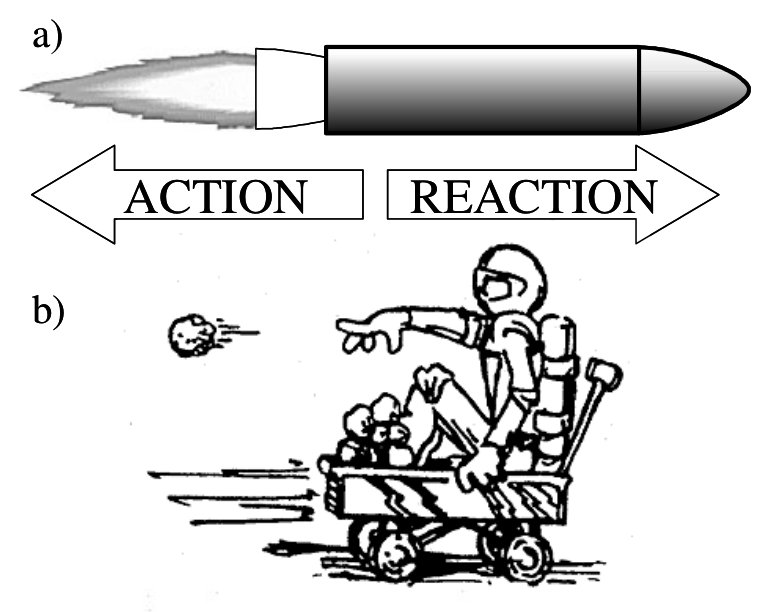
\includegraphics[scale=0.2]{cartoon.png}
\caption{Here Goes Your Figure's Caption.}
\label{fig:some_cartoon}
\end{center}
\end{figure}         
\\

A sample equation is written as:
\begin{equation} 
F_m=\frac{dm}{dt}v_e =  \dot{m}v_e 
\end{equation}


where m & is the mass flow rate and v e is the exit or exhaust velocity of the
propellant. 

An another sample equation can be expressed as

\begin{equation} F_m= \dot{m}v_e + (P_e - P_a)A_e \end{equation}

where $p_e$ and $A_e$ are the pressure and cross section area at the nozzle exit, and $p_a$ is
the ambient pressure.


\newpage
\section{Conclusion}
CONCLUSION, IF ANY.

\newpage
\section{Future Work}
FUTURE WORK, IF ANY

\newpage
\begin{thebibliography}
      
\bibitem{paperauthor1}
Humble R W, Henry G N and Larson W J (1995), \emph{Space propulsion analysis and design}, McGraw-Hill, Inc., ISBN-0-07-
031329-6.

\bibitem{FirstauthorYear}
Author First, Author Second \emph{Title of the paper} Name of Journal Page-numbers,
Month Year.


\end{thebibliography}

\end{document}

